\documentclass[a4paper]{article}
\renewcommand{\epsilon}{\varepsilon}
\newcommand{\triposcourse}{Analysis and Topology}
\usepackage{fancyhdr,titlesec,geometry}
\usepackage[dvipsnames]{xcolor}
\usepackage[many]{tcolorbox}
\usepackage{xifthen}
\usepackage{import}
\usepackage{parskip}
\usepackage{transparent}
\usepackage{mathtools,amssymb,amsfonts,amsthm,bm}   % Math Presets
\usepackage{array,tabularx,booktabs}                % Table Presets
\usepackage{graphicx,wrapfig,float,caption}         % Figure Presets
\usepackage{setspace,multicol}                      % Text Presets
\usepackage{tikz,physics,cancel,tkz-euclide,pgfplots,tikz-3dplot}                    % Physics Presets
\usepackage{amsmath}
\usepackage{mathrsfs}
\usepackage{enumerate}
\usepackage[shortlabels]{enumitem}
\usepackage{hyperref}
\usepackage{lipsum}
\usepackage{IEEEtrantools}
\usepackage{xcomment}
\usepackage{sectsty}
\usepackage{thmtools}
\usepackage{mdframed}
\usepackage{siunitx}
\usepackage{centernot}

\newcommand{\sectionbreak}{\clearpage}

\tdplotsetmaincoords{60}{120}

\usetikzlibrary{arrows.meta}
\usetikzlibrary{decorations.markings}
\usetikzlibrary{decorations.pathmorphing}
\usetikzlibrary{automata, positioning}
\usetikzlibrary{fadings}
\usetikzlibrary{intersections}
\usetikzlibrary{cd}
\usetikzlibrary{patterns}
\usetikzlibrary{shapes.arrows}
\usepgfplotslibrary{colormaps, external}
\pgfarrowsdeclarecombine{twolatex'}{twolatex'}{latex'}{latex'}{latex'}{latex'}
\tikzset{->/.style = {decoration={markings,
                                  mark=at position 1 with {\arrow[scale=1.6]{latex'}}},
                      postaction={decorate}}}
\tikzset{<-/.style = {decoration={markings,
                                  mark=at position 0 with {\arrowreversed[scale=1.6]{latex'}}},
                      postaction={decorate}}}
\tikzset{<->/.style = {decoration={markings,
                                   mark=at position 0 with {\arrowreversed[scale=1.6]{latex'}},
                                   mark=at position 1 with {\arrow[scale=1.6]{latex'}}},
                       postaction={decorate}}}
\tikzset{->-/.style = {decoration={markings,
                                   mark=at position #1 with {\arrow[scale=1.6]{latex'}}},
                       postaction={decorate}}}
\tikzset{-<-/.style = {decoration={markings,
                                   mark=at position #1 with {\arrowreversed[scale=1.6]{latex'}}},
                       postaction={decorate}}}
\tikzset{->>/.style = {decoration={markings,
                                  mark=at position 1 with {\arrow[scale=1.6]{twolatex'}}},
                      postaction={decorate}}}
\tikzset{<<-/.style = {decoration={markings,
                                  mark=at position 0 with {\arrowreversed[scale=1.6]{twolatex'}}},
                      postaction={decorate}}}
\tikzset{<<->>/.style = {decoration={markings,
                                   mark=at position 0 with {\arrowreversed[scale=1.6]{twolatex'}},
                                   mark=at position 1 with {\arrow[scale=1.6]{twolatex'}}},
                       postaction={decorate}}}
\tikzset{->>-/.style = {decoration={markings,
                                   mark=at position #1 with {\arrow[scale=1.6]{twolatex'}}},
                       postaction={decorate}}}
\tikzset{-<<-/.style = {decoration={markings,
                                   mark=at position #1 with {\arrowreversed[scale=1.6]{twolatex'}}},
                       postaction={decorate}}}

\tikzset{
set arrow inside/.code={\pgfqkeys{/tikz/arrow inside}{#1}},
set arrow inside={end/.initial=>, opt/.initial=},
/pgf/decoration/Mark/.style={
    mark/.expanded=at position #1 with
    {
        \noexpand\arrow[\pgfkeysvalueof{/tikz/arrow inside/opt}]{\pgfkeysvalueof{/tikz/arrow inside/end}}
    }
},
arrow inside/.style 2 args={
    set arrow inside={#1},
    postaction={
        decorate,decoration={
            markings,Mark/.list={#2}
        }
    }
},
}

\tikzstyle{circ}=[fill=black, draw=black, shape=circle]
\tikzset{
dot/.style = {circle, fill, minimum size=#1,
              inner sep=0pt, outer sep=0pt},
dot/.default = 5pt% size of the circle diameter 
}
\tikzset{mstate/.style={circle, draw, blue, text=black, minimum width=0.7cm}}
\tikzset{snake it/.style={-stealth,
decoration={snake, 
    amplitude = .4mm,
    segment length = 2mm,
    post length=0.9mm},decorate}}

\def\centerarc[#1](#2)(#3:#4:#5)% Syntax: [draw options](center)(initial angle:final angle:radius)
    { \draw[#1] ($(#2)+({#5*cos(#3)},{#5*sin(#3)})$) arc (#3:#4:#5); }

\hypersetup{
    colorlinks=true,
    linkcolor=blue,
    filecolor=blue,
    citecolor = black,      
    urlcolor=cyan,
    }

%%%%%%%%%%% Snippets %%%%%%%%%%%%%%%%
\newcommand*\widefbox[1]{\fbox{\hspace{2em}#1\hspace{2em}}}
\newcommand{\xint}{\int_{x_1}^{x_2}}
\newcommand{\mw}{\sqrt{m\omega}}
\newcommand{\de}{\delta}
\newcommand{\dde}{\dot{\delta}}
\newcommand{\di}{\delta_i}
\newcommand{\ddi}{\dot{\delta_i}}
\newcommand{\dddi}{\ddot{\delta_i}}
\newcommand{\dipl}{\delta_{i+1}}
\newcommand{\dimi}{\delta_{i-1}}
\newcommand{\ddt}[1]{\frac{{d} #1}{dt}}
\newcommand{\ddtt}[1]{\frac{d^2 #1}{dt^2}}
\newcommand{\ddx}[1]{\frac{d #1}{dx}}
\newcommand{\ddxx}[1]{\frac{d^2 #1}{dx^2}}
\newcommand{\eps}{\epsilon}
\newcommand{\del}[2]{\frac{\partial #1}{\partial #2}}
\newcommand{\deltwo}[2]{\frac{\partial^2 #1}{\partial #2^2}}
\newcommand{\lam}{\lambda}
\newcommand{\Lam}{\Lambda}
\newcommand{\sig}{\sigma}
\newcommand{\Sig}{\Sigma}
\newcommand{\half}{\frac{1}{2}}
\newcommand{\munu}{{\mu\nu}}
\newcommand{\thalf}{\tfrac{1}{2}}
\renewcommand{\div}{\nabla\cdot}
\renewcommand{\curl}{\nabla\times}

\DeclareMathOperator{\orb}{Orb}
\DeclareMathOperator{\stab}{Stab}
\DeclareMathOperator{\adj}{adj}
\DeclareMathOperator{\ccl}{ccl}
\let\var\relax
\DeclareMathOperator{\var}{Var}
\DeclareMathOperator{\cov}{Cov}
\DeclareMathOperator{\corr}{Corr}
\DeclareMathOperator{\Markov}{Markov}
\DeclareMathOperator{\nullity}{nullity}

\newcommand{\bfA}{{\bf A}}
\newcommand{\bfB}{{\bf B}}
\newcommand{\bfC}{{\bf C}}
\newcommand{\bfD}{{\bf D}}
\newcommand{\bfE}{{\bf E}}
\newcommand{\bfF}{{\bf F}}
\newcommand{\bfG}{{\bf G}}
\newcommand{\bfH}{{\bf H}}
\newcommand{\bfI}{{\bf I}}
\newcommand{\bfJ}{{\bf J}}
\newcommand{\bfK}{{\bf K}}
\newcommand{\bfL}{{\bf L}}
\newcommand{\bfM}{{\bf M}}
\newcommand{\bfN}{{\bf N}}
\newcommand{\bfO}{{\bf O}}
\newcommand{\bfP}{{\bf P}}
\newcommand{\bfQ}{{\bf Q}}
\newcommand{\bfR}{{\bf R}}
\newcommand{\bfS}{{\bf S}}
\newcommand{\bfT}{{\bf T}}
\newcommand{\bfU}{{\bf U}}
\newcommand{\bfV}{{\bf V}}
\newcommand{\bfW}{{\bf W}}
\newcommand{\bfX}{{\bf X}}
\newcommand{\bfY}{{\bf Y}}
\newcommand{\bfZ}{{\bf Z}}

\newcommand{\bfa}{{\bf a}}
\newcommand{\bfb}{{\bf b}}
\newcommand{\bfc}{{\bf c}}
\newcommand{\bfd}{{\bf d}}
\newcommand{\bfe}{{\bf e}}
\newcommand{\bff}{{\bf f}}
\newcommand{\bfg}{{\bf g}}
\newcommand{\bfh}{{\bf h}}
\newcommand{\bfi}{{\bf i}}
\newcommand{\bfj}{{\bf j}}
\newcommand{\bfk}{{\bf k}}
\newcommand{\bfl}{{\bf l}}
\newcommand{\bfm}{{\bf m}}
\newcommand{\bfn}{{\bf n}}
\newcommand{\bfo}{{\bf o}}
\newcommand{\bfp}{{\bf p}}
\newcommand{\bfq}{{\bf q}}
\newcommand{\bfr}{{\bf r}}
\newcommand{\bfs}{{\bf s}}
\newcommand{\bft}{{\bf t}}
\newcommand{\bfu}{{\bf u}}
\newcommand{\bfv}{{\bf v}}
\newcommand{\bfw}{{\bf w}}
\newcommand{\bfx}{{\bf x}}
\newcommand{\bfy}{{\bf y}}
\newcommand{\bfz}{{\bf z}}

\newcommand{\mcA}{{\mathcal{A}}}
\newcommand{\mcB}{{\mathcal{B}}}
\newcommand{\mcC}{{\mathcal{C}}}
\newcommand{\mcD}{{\mathcal{D}}}
\newcommand{\mcE}{{\mathcal{E}}}
\newcommand{\mcF}{{\mathcal{F}}}
\newcommand{\mcG}{{\mathcal{G}}}
\newcommand{\mcH}{{\mathcal{H}}}
\newcommand{\mcI}{{\mathcal{I}}}
\newcommand{\mcJ}{{\mathcal{J}}}
\newcommand{\mcK}{{\mathcal{K}}}
\newcommand{\mcL}{{\mathcal{L}}}
\newcommand{\mcM}{{\mathcal{M}}}
\newcommand{\mcN}{{\mathcal{N}}}
\newcommand{\mcO}{{\mathcal{O}}}
\newcommand{\mcP}{{\mathcal{P}}}
\newcommand{\mcQ}{{\mathcal{Q}}}
\newcommand{\mcR}{{\mathcal{R}}}
\newcommand{\mcS}{{\mathcal{S}}}
\newcommand{\mcT}{{\mathcal{T}}}
\newcommand{\mcU}{{\mathcal{U}}}
\newcommand{\mcV}{{\mathcal{V}}}
\newcommand{\mcW}{{\mathcal{W}}}
\newcommand{\mcX}{{\mathcal{X}}}
\newcommand{\mcY}{{\mathcal{Y}}}
\newcommand{\mcZ}{{\mathcal{Z}}}

\newcommand{\bbA}{{\mathbb{A}}}
\newcommand{\bbB}{{\mathbb{B}}}
\newcommand{\bbC}{{\mathbb{C}}}
\newcommand{\bbD}{{\mathbb{D}}}
\newcommand{\bbE}{{\mathbb{E}}}
\newcommand{\bbF}{{\mathbb{F}}}
\newcommand{\bbG}{{\mathbb{G}}}
\newcommand{\bbH}{{\mathbb{H}}}
\newcommand{\bbI}{{\mathbb{I}}}
\newcommand{\bbJ}{{\mathbb{J}}}
\newcommand{\bbK}{{\mathbb{K}}}
\newcommand{\bbL}{{\mathbb{L}}}
\newcommand{\bbM}{{\mathbb{M}}}
\newcommand{\bbN}{{\mathbb{N}}}
\newcommand{\bbO}{{\mathbb{O}}}
\newcommand{\bbP}{{\mathbb{P}}}
\newcommand{\bbQ}{{\mathbb{Q}}}
\newcommand{\bbR}{{\mathbb{R}}}
\newcommand{\bbS}{{\mathbb{S}}}
\newcommand{\bbT}{{\mathbb{T}}}
\newcommand{\bbU}{{\mathbb{U}}}
\newcommand{\bbV}{{\mathbb{V}}}
\newcommand{\bbW}{{\mathbb{W}}}
\newcommand{\bbX}{{\mathbb{X}}}
\newcommand{\bbY}{{\mathbb{Y}}}
\newcommand{\bbZ}{{\mathbb{Z}}}

\newcommand{\mfa}{{\mathfrak{a}}}
\newcommand{\mfb}{{\mathfrak{b}}}
\newcommand{\mfc}{{\mathfrak{c}}}
\newcommand{\mfd}{{\mathfrak{d}}}
\newcommand{\mfe}{{\mathfrak{e}}}
\newcommand{\mff}{{\mathfrak{f}}}
\newcommand{\mfg}{{\mathfrak{g}}}
\newcommand{\mfh}{{\mathfrak{h}}}
\newcommand{\mfi}{{\mathfrak{i}}}
\newcommand{\mfj}{{\mathfrak{j}}}
\newcommand{\mfk}{{\mathfrak{k}}}
\newcommand{\mfl}{{\mathfrak{l}}}
\newcommand{\mfm}{{\mathfrak{m}}}
\newcommand{\mfn}{{\mathfrak{n}}}
\newcommand{\mfo}{{\mathfrak{o}}}
\newcommand{\mfp}{{\mathfrak{p}}}
\newcommand{\mfq}{{\mathfrak{q}}}
\newcommand{\mfr}{{\mathfrak{r}}}
\newcommand{\mfs}{{\mathfrak{s}}}
\newcommand{\mft}{{\mathfrak{t}}}
\newcommand{\mfu}{{\mathfrak{u}}}
\newcommand{\mfv}{{\mathfrak{v}}}
\newcommand{\mfw}{{\mathfrak{w}}}
\newcommand{\mfx}{{\mathfrak{x}}}
\newcommand{\mfy}{{\mathfrak{y}}}
\newcommand{\mfz}{{\mathfrak{z}}}

\newcommand{\mfA}{{\mathfrak{A}}}
\newcommand{\mfB}{{\mathfrak{B}}}
\newcommand{\mfC}{{\mathfrak{C}}}
\newcommand{\mfD}{{\mathfrak{D}}}
\newcommand{\mfE}{{\mathfrak{E}}}
\newcommand{\mfF}{{\mathfrak{F}}}
\newcommand{\mfG}{{\mathfrak{G}}}
\newcommand{\mfH}{{\mathfrak{H}}}
\newcommand{\mfI}{{\mathfrak{I}}}
\newcommand{\mfJ}{{\mathfrak{J}}}
\newcommand{\mfK}{{\mathfrak{K}}}
\newcommand{\mfL}{{\mathfrak{L}}}
\newcommand{\mfM}{{\mathfrak{M}}}
\newcommand{\mfN}{{\mathfrak{N}}}
\newcommand{\mfO}{{\mathfrak{O}}}
\newcommand{\mfP}{{\mathfrak{P}}}
\newcommand{\mfQ}{{\mathfrak{Q}}}
\newcommand{\mfR}{{\mathfrak{R}}}
\newcommand{\mfS}{{\mathfrak{S}}}
\newcommand{\mfT}{{\mathfrak{T}}}
\newcommand{\mfU}{{\mathfrak{U}}}
\newcommand{\mfV}{{\mathfrak{V}}}
\newcommand{\mfW}{{\mathfrak{W}}}
\newcommand{\mfX}{{\mathfrak{X}}}
\newcommand{\mfY}{{\mathfrak{Y}}}
\newcommand{\mfZ}{{\mathfrak{Z}}}

\newcommand{\rma}{\mathrm{a}}
\newcommand{\rmb}{\mathrm{b}}
\newcommand{\rmc}{\mathrm{c}}
\newcommand{\rmd}{\mathrm{d}}
\renewcommand{\dd}{\,\mathrm{d}}
\newcommand{\rme}{\mathrm{e}}
\newcommand{\rmf}{\mathrm{f}}
\newcommand{\rmg}{\mathrm{g}}
\newcommand{\rmh}{\mathrm{h}}
\newcommand{\rmi}{\mathrm{i}}
\newcommand{\rmj}{\mathrm{j}}
\newcommand{\rmk}{\mathrm{k}}
\newcommand{\rml}{\mathrm{l}}
\newcommand{\rmm}{\mathrm{m}}
\newcommand{\rmn}{\mathrm{n}}
\newcommand{\rmo}{\mathrm{o}}
\newcommand{\rmp}{\mathrm{p}}
\newcommand{\rmq}{\mathrm{q}}
\newcommand{\rmr}{\mathrm{r}}
\newcommand{\rms}{\mathrm{s}}
\newcommand{\rmt}{\mathrm{t}}
\newcommand{\rmu}{\mathrm{u}}
\newcommand{\rmv}{\mathrm{v}}
\newcommand{\rmw}{\mathrm{w}}
\newcommand{\rmx}{\mathrm{x}}
\newcommand{\rmy}{\mathrm{y}}
\newcommand{\rmz}{\mathrm{z}}
\newcommand{\rmA}{\mathrm{A}}
\newcommand{\rmB}{\mathrm{B}}
\newcommand{\rmC}{\mathrm{C}}
\newcommand{\rmD}{\mathrm{D}}
\newcommand{\rmE}{\mathrm{E}}
\newcommand{\rmF}{\mathrm{F}}
\newcommand{\rmG}{\mathrm{G}}
\newcommand{\rmH}{\mathrm{H}}
\newcommand{\rmI}{\mathrm{I}}
\newcommand{\rmJ}{\mathrm{J}}
\newcommand{\rmK}{\mathrm{K}}
\newcommand{\rmL}{\mathrm{L}}
\newcommand{\rmM}{\mathrm{M}}
\newcommand{\rmN}{\mathrm{N}}
\newcommand{\rmO}{\mathrm{O}}
\newcommand{\rmP}{\mathrm{P}}
\newcommand{\rmQ}{\mathrm{Q}}
\newcommand{\rmR}{\mathrm{R}}
\newcommand{\rmS}{\mathrm{S}}
\newcommand{\rmT}{\mathrm{T}}
\newcommand{\rmU}{\mathrm{U}}
\newcommand{\rmV}{\mathrm{V}}
\newcommand{\rmW}{\mathrm{W}}
\newcommand{\rmX}{\mathrm{X}}
\newcommand{\rmY}{\mathrm{Y}}
\newcommand{\rmZ}{\mathrm{Z}}

\newcommand{\GL}{\mathrm{GL}}
\newcommand{\Or}{\mathrm{O}}
\newcommand{\PGL}{\mathrm{PGL}}
\newcommand{\PSL}{\mathrm{PSL}}
\newcommand{\PSO}{\mathrm{PSO}}
\newcommand{\PSU}{\mathrm{PSU}}
\newcommand{\SL}{\mathrm{SL}}
\newcommand{\SO}{\mathrm{SO}}
\newcommand{\Spin}{\mathrm{Spin}}
\newcommand{\Sp}{\mathrm{Sp}}
\newcommand{\SU}{\mathrm{SU}}
\newcommand{\Mat}{\mathrm{Mat}}

% Some common notations

\renewcommand{\v}{\mathbf{v}}
\newcommand{\w}{\mathbf{w}}
\renewcommand{\u}{\mathbf{u}}

% Matrix algebras
\newcommand{\gl}{\mathfrak{gl}}
\newcommand{\ort}{\mathfrak{o}}
\newcommand{\so}{\mathfrak{so}}
\newcommand{\su}{\mathfrak{su}}
\newcommand{\uu}{\mathfrak{u}}
\renewcommand{\sl}{\mathfrak{sl}}
\newcommand{\inner}[1]{\left\langle{#1}\right\rangle}
\DeclareMathOperator{\spn}{span}

\newcommand{\mobius}{{M\"{o}bius }}

\renewcommand{\ge}{\geqslant}
\renewcommand{\le}{\leqslant}
\renewcommand{\geq}{\geqslant}
\renewcommand{\leq}{\leqslant}
\renewcommand{\restriction}{\mathord{\upharpoonright}}

\newcommand\independent{\protect\mathpalette{\protect\independenT}{\perp}}
\def\independenT#1#2{\mathrel{\rlap{$#1#2$}\mkern2mu{#1#2}}}

\setlength{\parindent}{0pt}
% \setlength{\parskip}{\baselineskip}
\newcommand{\incfig}[1]{%
    \def\svgwidth{0.4\columnwidth}
    \import{./figures/}{#1.pdf_tex}
}
%%%%%%%%%%%%%%%%%%%%%%%%%%%%%%%%%%%%%

\usepackage[T1]{fontenc}
\usepackage{lmodern,mathrsfs}

%%%%%%%boxed enviroment for final layout%%%%%%%%%%%%%

\newtheoremstyle{mystyle}%
  {}%
  {}%
  {}%
  {}%
  {\sffamily\bfseries}%
  {.}%
  { }%
  {}%

% \renewenvironment{proof}{{\sffamily\bfseries Proof. }}{\qed}

\theoremstyle{mystyle}{
  \newtheorem{theorem}{Theorem}[section]
  \newtheorem{lemma}[theorem]{Lemma}
  \newtheorem{proposition}[theorem]{Proposition}
  \newtheorem{corollary}[theorem]{Corollary}
  \newtheorem{problem}[theorem]{Problem}
  \newtheorem*{claim}{Claim}
  \newtheorem*{slemma}{Lemma}
  \newtheorem*{sprop}{Proposition}
  \newtheorem*{notation}{Notation}

  \newtheorem{inquestion}{Question}
  \newtheorem*{sque}{Question}

  \newtheorem{definition}{Definition}[section]
  \newtheorem{conjecture}{Conjecture}[section]
  \newtheorem{example}{Example}[section]
  \newtheorem*{law}{Law}

  \newtheorem*{remark}{Remark}
  \newtheorem*{note}{Note}
}

\newenvironment{question}[1]
{\renewcommand\theinquestion{#1}\inquestion}
{\endinquestion}

\theoremstyle{definition}{
    \newtheorem*{exercise}{Exercise}}

\tcolorboxenvironment{definition}{
  boxrule=0pt,
  boxsep=2pt,
  colback={White!90!Cerulean},
  enhanced jigsaw, 
  borderline west={2pt}{0pt}{Cerulean},
  sharp corners,
  before skip=10pt,
  after skip=10pt,
  breakable,
  % parbox=false,
}

\tcolorboxenvironment{notation}{
  boxrule=0pt,
  boxsep=2pt,
  colback={White!90!Cerulean},
  enhanced jigsaw, 
  borderline west={2pt}{0pt}{Cerulean},
  sharp corners,
  before skip=10pt,
  after skip=10pt,
  breakable,
  % parbox=false,
}

\tcolorboxenvironment{proposition}{
  boxrule=0pt,
  boxsep=2pt,
  colback={White!90!Yellow},
  enhanced jigsaw, 
  borderline west={2pt}{0pt}{Yellow},
  sharp corners,
  before skip=10pt,
  after skip=10pt,
  breakable,
  % parbox=false,
}

\tcolorboxenvironment{sprop}{
  boxrule=0pt,
  boxsep=2pt,
  colback={White!90!Yellow},
  enhanced jigsaw, 
  borderline west={2pt}{0pt}{Yellow},
  sharp corners,
  before skip=10pt,
  after skip=10pt,
  breakable,
  % parbox=false,
}

\tcolorboxenvironment{theorem}{
  boxrule=0pt,
  boxsep=2pt,
  colback={White!90!Dandelion},
  enhanced jigsaw, 
  borderline west={2pt}{0pt}{Dandelion},
  sharp corners,
  before skip=10pt,
  after skip=10pt,
  breakable,
  % parbox=false,
}

\tcolorboxenvironment{lemma}{
  boxrule=0pt,
  boxsep=2pt,
  blanker,
  borderline west={2pt}{0pt}{Red},
  before skip=10pt,
  after skip=10pt,
  sharp corners,
  left=12pt,
  right=12pt,
  breakable,
  % parbox=false,
}

\tcolorboxenvironment{corollary}{
  boxrule=0pt,
  boxsep=2pt,
  blanker,
  borderline west={2pt}{0pt}{ForestGreen},
  before skip=10pt,
  after skip=10pt,
  sharp corners,
  left=12pt,
  right=12pt,
  breakable,
  % parbox=false,
}

\tcolorboxenvironment{proof}{
  boxrule=0pt,
  boxsep=2pt,
  blanker,
  borderline west={2pt}{0pt}{NavyBlue!80!white},
  before skip=10pt,
  after skip=10pt,
  left=12pt,
  right=12pt,
  breakable,
  % parbox=false,
}

\tcolorboxenvironment{remark}{
  boxrule=0pt,
  boxsep=2pt,
  blanker,
  borderline west={2pt}{0pt}{Green},
  before skip=10pt,
  after skip=10pt,
  left=12pt,
  right=12pt,
  breakable,
  % parbox=false,
}

\tcolorboxenvironment{note}{
  boxrule=0pt,
  boxsep=2pt,
  blanker,
  borderline west={2pt}{0pt}{PineGreen},
  before skip=10pt,
  after skip=10pt,
  left=12pt,
  right=12pt,
  breakable,
  % parbox=false,
}

\tcolorboxenvironment{example}{
  boxrule=0pt,
  boxsep=2pt,
  blanker,
  borderline west={2pt}{0pt}{Black},
  sharp corners,
  before skip=10pt,
  after skip=10pt,
  left=12pt,
  right=12pt,
  breakable,
  % parbox=false,
}

\titleformat*{\section}{\Large\bfseries\sffamily}
\titleformat*{\subsection}{\large\bfseries\sffamily}
\titleformat*{\subsubsection}{\bfseries\sffamily}
\titleformat*{\paragraph}{\bfseries\sffamily}

%%%%%%%%%%%%%%%%%%%%%%%%%%%%%%%%%%%%%%%%%%%%%%%%%%%%

\title{\textbf{\sffamily\triposcourse{} Notes}}
% \usepackage[T1]{fontenc}
\usepackage{crimson}

\theoremstyle{plain}

\theoremstyle{definition}
\newtheorem{theorem}{Theorem}[section]
\newtheorem{lemma}[theorem]{Lemma}
\newtheorem{proposition}[theorem]{Proposition}
\newtheorem{corollary}[theorem]{Corollary}
\newtheorem{problem}[theorem]{Problem}
\newtheorem*{claim}{Claim}
\newtheorem*{slemma}{Lemma}
\newtheorem*{sprop}{Proposition}
\newtheorem*{notation}{Notation}
\newtheorem*{exercise}{Exercise}

\newtheorem{inquestion}{Question}
\newtheorem*{sque}{Question}
\newenvironment{question}[1]
  {\renewcommand\theinquestion{#1}\inquestion}
  {\endinquestion}

\newtheorem{definition}{Definition}[section]
\newtheorem{conjecture}{Conjecture}[section]
\newtheorem{example}{Example}[section]
\newtheorem*{law}{Law}

\theoremstyle{remark}
\newtheorem*{remark}{Remark}
\newtheorem*{note}{Note}

\title{\textbf{\triposcourse{} Notes}}
% \theoremstyle{plain}{
  \newtheorem{theorem}{Theorem}[section]
  \newtheorem{lemma}[theorem]{Lemma}
  \newtheorem{proposition}[theorem]{Proposition}
  \newtheorem{corollary}[theorem]{Corollary}
  \newtheorem*{claim}{Claim}
  \newtheorem*{slemma}{Lemma}
  \newtheorem*{sprop}{Proposition}
  \newtheorem{conjecture}{Conjecture}[section]
  \newtheorem*{law}{Law}
  \newtheorem{inquestion}{Question}
  \newtheorem*{sque}{Question}
}

\theoremstyle{definition}{
  \newtheorem{method}[theorem]{Method}
  \newtheorem{definition}{Definition}[section]
  \newtheorem{example}{Example}[section]
  \newtheorem*{notation}{Notation}
  \newtheorem*{exercise}{Exercise}
}

\theoremstyle{remark}{
  \newtheorem{remark}[theorem]{Remark}
  \newtheorem*{note}{Note}
}

\newenvironment{question}[1]
{\renewcommand\theinquestion{#1}\inquestion}
{\endinquestion}

\title{\textbf{\sffamily\triposcourse{} Notes}}

%layout full
% \geometry{%
%   a4paper,
%   lmargin=2cm,
%   rmargin=2.5cm,
%   tmargin=3.5cm,
%   bmargin=2.5cm,
%   footskip=12pt,
%   headheight=24pt}
% layout trim
% \geometry{
% papersize={379pt, 542pt},
% textwidth=345pt,
% textheight=443pt,
% left=17pt,
% top=54pt,
% right=17pt
% }
% layout a5
\geometry{%
  a5paper,
  lmargin=1cm,
  rmargin=1cm,
  tmargin=2.5cm,
  bmargin=1.5cm,
  footskip=15pt,
  headheight=24pt}
\pagestyle{fancy}
\rhead{{\triposcourse{}}}
\author{jt775}
\AddToHook{cmd/section/before}{\clearpage}

\graphicspath{ {./images/} }
\pgfplotsset{compat=1.17}
\begin{document}
\maketitle
\tableofcontents
\newpage
\part*{Lecture 1}
\section{Uniform convergence and uniform continuity}
\subsection{Pointwise and uniform convergence}
Recall that in $\mathbb{R}$ or $\mathbb{C}$ we write $x_{n} \rightarrow x$ as $n \rightarrow \infty$ if
\[
\forall \varepsilon>0 \quad \exists N \in \mathbb{N} \quad \forall n \geqslant N \quad\left|x_{n}-x\right|<\varepsilon
\]
The aim is to define $f_{n} \rightarrow f$ for functions $f_{n}$ and $f$.

\begin{definition}
    We have a set $S$ and functions $f_{n}: S \rightarrow \mathbb{R}, n \in \mathbb{N}$, and $f: S \rightarrow \mathbb{R}$. Then $f_{n} \rightarrow f$ pointwise on $S$ as $n \rightarrow \infty$ if for every $x \in S$, the real sequence $\left(f_{n}(x)\right)_{n}$ converges to $f(x)$. In symbols:
    \[
    \forall x \in S \quad \forall \varepsilon>0 \quad \exists N \in \mathbb{N} \quad \forall n \geqslant N \quad\left|f_{n}(x)-f(x)\right|<\varepsilon
    \]
\end{definition}

\begin{remark}\
    \begin{enumerate}
        \item  $N$ can depend on $\varepsilon$ and $x$.
        \item Can replace $\mathbb{R}$ with $\mathbb{C}$.
        \item It is possible that $f_{n} \rightarrow f$ pointwise on some subset $T \subset S$. In the definition replace $\forall x \in S$ with $\forall x \in T$.
        \item The pointwise limit of a sequence of functions $(f_n)$ is unique if it exists.
    \end{enumerate}
\end{remark}

\begin{example}\
    \begin{enumerate}
        \item $f_{n}(x)=x^{n}$ for $x \in[0,1], n \in \mathbb{N}$.
        
        For $0 \leqslant x<1$, we have $f_{n}(x)=x^{n} \rightarrow 0$ as $n \rightarrow \infty$.
        Also, $f_{n}(1)=1 \rightarrow 1$ as $n \rightarrow \infty$. So $f_{n} \rightarrow f$ pointwise on $[0,1]$, where
        \[
        f(x)= \begin{cases}0 & \text { if } 0 \leqslant x<1 \\ 1 & \text { if } x=1\end{cases}
        \]
        \item $f_{n}(x)=x^{2} \cdot e^{-n x}$ for $x \in[0, \infty)$, and $n \in \mathbb{N}$. For $x>0$
        \[
        0 \leqslant f_{n}(x)=\frac{x^{2}}{e^{n x}}=\frac{x^{2}}{1+n x+\frac{n^{2} x^{2}}{2}+\ldots} \leqslant \frac{x^{2}}{n x}=\frac{x}{n}
        \]
        Hence $f_{n}(x) \rightarrow 0$ as $n \rightarrow \infty$. Same is true $x=0$. Thus, $f_{n} \rightarrow 0$ pointwise on $[0, \infty)$.
    \end{enumerate}
\end{example}

\begin{definition}
    We are given a set $S$ and functions $f_{n}: S \rightarrow \mathbb{R}, n \in \mathbb{N}$, and $f: S \rightarrow \mathbb{R}$. Then $f_{n} \rightarrow f$ uniformly on $S$ as $n \rightarrow \infty$ if
    \[
    \forall \varepsilon>0 \quad \exists N \in \mathbb{N} \quad \forall n \geqslant N \quad \forall x \in S \quad\left|f_{n}(x)-f(x)\right|<\varepsilon
    \]
    \begin{center}
        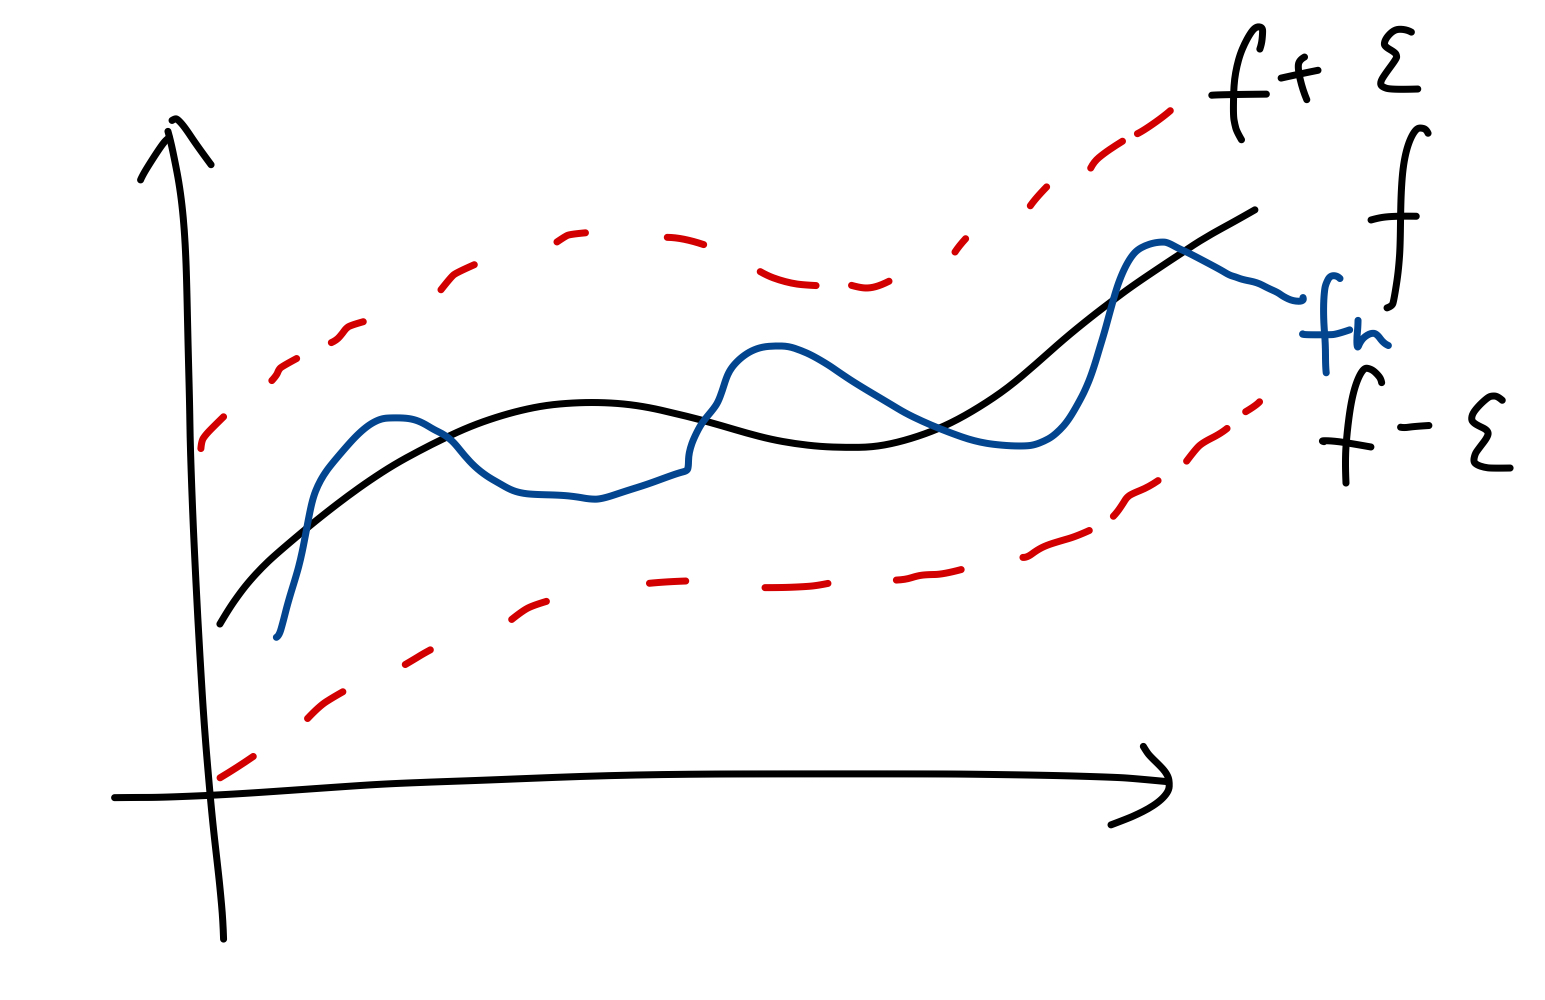
\includegraphics[scale=0.11]{at1.jpeg}
    \end{center}
\end{definition}

\begin{remark}\
    \begin{enumerate}
        \item $ N $ only depends on $\epsilon$!
        \item Uniform convergence implies pointwise convergence.
        \item Can replace $\mathbb{R}$ with $\mathbb{C}$ and can restrict to a subset of the domain.
        \item An equivalent definition of $f_{n} \rightarrow f$ uniformly on $S$ :
        \[
        \forall \varepsilon>0 \quad \exists N \in \mathbb{N} \quad \forall n \geqslant N \quad \sup _{x \in S}\left|f_{n}(x)-f(x)\right|<\varepsilon
        \]
        Even shorter: $\sup _{x \in S}\left|f_{n}(x)-f(x)\right| \rightarrow 0$ as $n \rightarrow \infty$
        \item The uniform limit $f$ if exists is unique.
    \end{enumerate}
\end{remark}

\begin{example}
\begin{enumerate}
    \item $f_{n}(x)=x^{2} \cdot e^{-n x}$ for $x \in[0, \infty)$, and $n \in \mathbb{N}$. We saw that $f_{n} \rightarrow f=0$ pointwise on $[0, \infty)$.
    \[
    0 \leqslant f_{n}(x)=\frac{x^{2}}{e^{n x}}=\frac{x^{2}}{1+n x+\frac{n^{2} x^{2}}{2}+\ldots} \leqslant \frac{2}{n^2}
    \]
    Thus,
    \[
    \sup _{x \in[0, \infty)}\left|f_{n}(x)-f(x)\right|=\sup _{x \in[0, \infty)} f_{n}(x) \leqslant \frac{2}{n^{2}} \rightarrow 0 \quad \text { as } \quad n \rightarrow \infty
    \]
    So $f_{n} \rightarrow 0$ uniformly on $[0, \infty)$.

    Could have used differentiation above to find the supremum, but the above method of finding an upper bound is better.
    \item $f_{n}(x)=x^{n}$ for $x \in[0,1], n \in \mathbb{N}$.
    We know that $f_{n} \rightarrow f$ pointwise on $[0,1]$, where
    \[
        f(x)= \begin{cases}0 & \text { if } 0 \leqslant x<1 \\ 1 & \text { if } x=1\end{cases}.
    \]
    Let $\varepsilon=1 / 2$. For any $n \in \mathbb{N}$, setting $x=\varepsilon^{1 / n}$, we have $f_{n}(x)=\varepsilon$, and so $\left|f_{n}(x)-f(x)\right| \geqslant \varepsilon$. So $f_{n} \not \rightarrow  f$ uniformly on $[0,1]$.

    Better: Since $f_{n}(1)=1$ and $f_{n}$ is continuous, there exist $\delta>0$ such that $\left|f_{n}(x)-1\right|<1 / 2$ for $x \in(1-\delta, 1+\delta)$. So for any $x \in[0,1]$ with $1-\delta<x<1$, we have $\left|f_{n}(x)-f(x)\right| \geqslant \varepsilon$.
\end{enumerate}
\end{example}

Q: Does $\left(f_{n}\right)$ converge uniformly on $S ?$
\subsubsection*{Strategy}
First check if $\left(f_{n}\right)$ converges pointwise on $S$.

If it doesn't, then $\left(f_{n}\right)$ does not converge uniformly on $S$.

If it does, then compute the pointwise limit $f$, and then it remains to check whether
\[
\sup _{x \in S}\left|f_{n}(x)-f(x)\right| \rightarrow 0 \quad \text { as } \quad n \rightarrow \infty
\]

If the above holds, then $f_{n} \rightarrow f$ uniformly on $S$, otherwise $\left(f_{n}\right)$ does not converge uniformly on $S$.

\begin{remark}
    What does it mean that $f_{n} \not \rightarrow f$ uniformly on $S$? We have to negate the sentence
    \[
    \forall \varepsilon>0 \quad \exists N \in \mathbb{N} \quad \forall n \geqslant N \quad \forall x \in S \quad\left|f_{n}(x)-f(x)\right|<\varepsilon
    \]
    The negation is
    \[
    \exists \varepsilon>0 \quad \forall N \in \mathbb{N} \quad \exists n \geqslant N \quad \exists x \in S \quad\left|f_{n}(x)-f(x)\right| \geqslant \varepsilon
    \]
\end{remark}
\newpage
\part*{Lecture 2}
\subsection{Continuity and boundedness}
The next theorem says that uniform limit of continuous functions is continuous.
\begin{theorem}\label{thm:1}
    Let $S$ be a subset of $\mathbb{R}$ or $\mathbb{C}$. Assume $f_{n} \rightarrow f$ uniformly on $S$. If $f_{n}$ is continuous for every $n \in \mathbb{N}$, then $f$ is continuous.
\end{theorem}

\textit{Idea}: Given $a \in S$, we want that $f(x) \approx f(a)$ provided $x \approx a$. We first choose large $n$ so that $f_{n}(x) \approx f(x)$ for every $x \in S$. Since $f_{n}$ is continuous, we have $f_{n}(x) \approx f_{n}(a)$ provided $x \approx a$. Thus, if $x \approx a$, then $f(x) \approx f_{n}(x) \approx f_{n}(a) \approx f(a)$.

\begin{proof}
    Fix $ a\in S, \epsilon>0 $. The goal is to find a $ \delta $ s.t. 
    \[
        \forall x\in S\quad |x-a|<\delta \Longrightarrow |f(x)-f(a)|<\epsilon.
    \]
    Since $ f_n\to f $ uniformly on $S$, $ \exists n\in \mathbb{N} $ such that 
    \[
        \forall x\in S\quad |f_n(x)-f(x)|<\epsilon.
    \]
    Since $f_n$ is continuous, $ \exists \delta>0 $, 
    \[
        \forall x\in S\quad |x-a|<\delta \Longrightarrow |f_n(x)-f_n(a)|<\epsilon.
    \]
    Thus for any $x\in S$, if $ |x-a|<\delta $,
    \[
        |f(x)-f(a)|\le |f(x)-f_n(x)|+|f_n(x)-f_n(a)|+|f_n(a)-f(a)|<3\epsilon.\qedhere
    \]
\end{proof}
\begin{remark}
    \begin{enumerate}
        \item It is not true for pointwise convergence. A counterexample is $x^n$.
        \item The result does not extend to differentiability.
        \item It follows from Theorem 1.1 that $x^{n}$ does not converge uniformly on $[0,1]$.
        \item The above proof is sometimes called a $3 \varepsilon$-proof.
        \item $\displaystyle \lim _{x \rightarrow a} \lim _{n \rightarrow \infty} f_{n}(x)=\lim _{x \rightarrow a} f(x)=f(a)=\lim _{n \rightarrow \infty} f_{n}(a)=\lim _{n \rightarrow \infty} \lim _{x \rightarrow a} f_{n}(x)$. i.e. we can \textit{swap limits} for uniformly convergent functions.
    \end{enumerate}
\end{remark}
\begin{lemma}\label{lemma 2}
    Let $S$ be any set and $f_{n}$ be a bounded function on $S$ for every $n \in \mathbb{N}$. If $f_{n} \rightarrow f$ uniformly on $S$, then $f$ is also bounded on $S$.
\end{lemma}
\begin{proof}
    Fix $n \in \mathbb{N}$ so that $\left|f_{n}(x)-f(x)\right| \leqslant 1$ for every $x \in S$. We can do this, since $f_{n} \rightarrow f$ uniformly on $S$. Since $f_{n}$ is bounded, there is an $M \in \mathbb{R}$ such that $\left|f_{n}(x)\right| \leqslant M$ for every $x \in S$. It follows that for every $x \in S$, we have
    \[
    |f(x)| \leqslant\left|f(x)-f_{n}(x)\right|+\left|f_{n}(x)\right| \leqslant 1+M
    \]
    Thus, $f$ is bounded by $M+1$.
\end{proof}
\subsection{Integrability and differentiability}

Before the next theorem, we recall some definitions and results from Analysis I. Assume $f:[a, b] \rightarrow \mathbb{R}$ is a bounded function. Given a dissection $\mathcal{D}: a=x_{0}<x_{1}<\cdots<x_{n}=b$ of $[a, b]$, the upper and lower sums of $f$ with respect to $\mathcal{D}$ are defined as
\[
U_{\mathcal{D}}(f)=\sum_{k=1}^{n}\left(x_{k}-x_{k-1}\right) \sup _{\left[x_{k-1}, x_{k}\right]} f \quad \text { and } \quad L_{\mathcal{D}}(f)=\sum_{k=1}^{n}\left(x_{k}-x_{k-1}\right) \inf _{\left[x_{k-1}, x_{k}\right]} f
\]
Riemann's criterion states that $f$ is integrable if and only if for every $\varepsilon>0$ there is a dissection $\mathcal{D}$ of $[a, b]$ such that
\[
U_{\mathcal{D}}(f)-L_{\mathcal{D}}(f)=\sum_{k=1}^{n}\left(x_{k}-x_{k-1}\right)\left(\sup _{\left[x_{k-1}, x_{k}\right]} f-\inf _{\left[x_{k-1}, x_{k}\right]} f\right)<\varepsilon
\]
An easy exercise shows that for an interval $I \subset[a, b]$ we have
\[
\sup _{I} f-\inf _{I} f=\sup _{x, y \in I}(f(x)-f(y))=\sup _{x, y \in I}|f(x)-f(y)|
\]
(This quantity is sometimes called the oscillation of $f$ on $I$.)

\begin{theorem}\label{theorem 3}
    Assume $f_{n}:[a, b] \rightarrow \mathbb{R}$ is Riemann-integrable for every $n \in \mathbb{N}$. If $f_{n} \rightarrow f$ uniformly on $[a, b]$, then $f$ is also Riemann-integrable on $[a, b]$, and moreover
    \[
    \int_{a}^{b} f_{n} \rightarrow \int_{a}^{b} f \quad \text { as } n \rightarrow \infty.
    \]
\end{theorem}
\begin{proof}
    We are going to prove that $f$ is bounded and that it satisfies Riemann's criterion. By definition of integrability, each $f_{n}$ is bounded, and hence so is $f$ by Lemma \ref{lemma 2}.
    Next, fix $\varepsilon>0$. Since $f_{n} \rightarrow f$ uniformly on $[a, b]$, we can fix $n \in \mathbb{N}$ so that $\left|f_{n}(x)-f(x)\right|<\varepsilon$ for all $x \in[a, b]$. Since $f_{n}$ is integrable, it satisfies Riemann's criterion, so there is a dissection $\mathcal{D}$ of $[a, b]$ such that $U_{\mathcal{D}}\left(f_{n}\right)-L_{\mathcal{D}}\left(f_{n}\right)<\varepsilon$. If $I$ is one of the sub-intervals of $\mathcal{D}$, then for any $x, y \in I$ we have
    \[
    \begin{aligned}
    |f(x)-f(y)| & \leqslant\left|f(x)-f_{n}(x)\right|+\left|f_{n}(x)-f_{n}(y)\right|+\left|f_{n}(y)-f(y)\right| \\
    &<\left|f_{n}(x)-f_{n}(y)\right|+2 \varepsilon
    \end{aligned}
    \]
    It follows that
    \[
    \sup _{x, y \in I}|f(x)-f(y)| \leqslant \sup _{x, y \in I}\left|f_{n}(x)-f_{n}(y)\right|+2 \varepsilon
    \]
    Multiplying both sides with the length of $I$ and summing over all sub-intervals $I$ of $\mathcal{D}$, we obtain
    \[
    U_{\mathcal{D}}(f)-L_{\mathcal{D}}(f) \leqslant U_{\mathcal{D}}\left(f_{n}\right)-L_{\mathcal{D}}\left(f_{n}\right)+2 \varepsilon(b-a)<(2(b-a)+1) \varepsilon.
    \]
    So $f$ satisfies Riemann's criterion, and thus, $f$ is integrable.
    Finally, we estimate
    \[
    \left|\int_{a}^{b} f_{n}-\int_{a}^{b} f\right| \leqslant \int_{a}^{b}\left|f_{n}-f\right| \leqslant(b-a) \sup _{[a, b]}\left|f_{n}-f\right| \rightarrow 0 \quad \text { as } n \rightarrow \infty .\qedhere
    \]
\end{proof}
\begin{remark}
    The conclusion of Theorem \ref{theorem 3} says: $\int_{a}^{b} \lim _{n \rightarrow \infty} f_{n}(x) \mathrm{d} x=\lim _{n \rightarrow \infty} \int_{a}^{b} f_{n}(x) \mathrm{d} x$. i.e. for uniformly convergent functions we can swap limits and integrals.
\end{remark}
\begin{corollary}\label{col:4}
    Let $f_{n}:[a, b] \rightarrow \mathbb{R}$ be an integrable function for each $n \in \mathbb{N}$. If $\sum_{n=1}^{\infty} f_{n}(x)$ converges uniformly on $[a, b]$, then $\sum_{n=1}^{\infty} f_{n}(x)$ defines an integrable function on $[a, b]$, and moreover
    \[
    \int_{a}^{b} \sum_{n=1}^{\infty} f_{n}(x) \mathrm{d} x=\sum_{n=1}^{\infty} \int_{a}^{b} f_{n}(x) \mathrm{d} x.
    \]
\end{corollary}
\begin{proof}
    Define $F_{n}(x)=\sum_{k=1}^{n} f_{k}(x)$ for $x \in[a, b]$ and $n \in \mathbb{N}$. To say that $\sum_{n=1}^{\infty} f_{n}(x)$ converges uniformly on $[a, b]$ means that $\left(F_{n}\right)$ converges uniformly on $[a, b]$. So for each $x \in[a, b]$, the series $\sum_{n=1}^{\infty} f_{n}(x)$ is convergent, and the function $x \mapsto \sum_{n=1}^{\infty} f_{n}(x)$ is the uniform limit of $\left(F_{n}\right)$ on $[a, b]$.

    We know that each $F_{n}$ is integrable and $\int_{a}^{b} F_{n}=\sum_{k=1}^{n} \int_{a}^{b} f_{k}$. So by Theorem 3 , the function $\sum_{n=1}^{\infty} f_{n}(x)$ is integrable and
    \[
    \int_{a}^{b} \sum_{n=1}^{\infty} f_{n}(x) \mathrm{d} x=\lim _{n \rightarrow \infty} \int_{a}^{b} F_{n}(x) \mathrm{d} x=\lim _{n \rightarrow \infty} \sum_{k=1}^{n} \int_{a}^{b} f_{k}(x) \mathrm{d} x=\sum_{k=1}^{\infty} \int_{a}^{b} f_{k}(x) \mathrm{d} x.\qedhere
    \]
\end{proof}
\begin{theorem}\label{thm:5}
    Let $\left(f_{n}\right)$ be a sequence of continuously differentiable functions on $[a, b]$. Assume further that
    \begin{enumerate}
        \item $\sum_{n=1}^{\infty} f_{n}^{\prime}(x)$ converges uniformly on $[a, b]$;
        \item there exists $c \in[a, b]$ such that $\sum_{n=1}^{\infty} f_{n}(c)$ converges.
    \end{enumerate}
    Then $\sum_{n=1}^{\infty} f_{n}(x)$ converges uniformly to a continuously differentiable function $f$ on $[a, b]$, and moreover, we have
    \[
    f^{\prime}(x)=\sum_{n=1}^{\infty} f_{n}^{\prime}(x) \quad \text { for all } x \in[a, b].
    \]
\end{theorem}
\begin{note}
    Informally, $\displaystyle \frac{\mathrm{d}}{\mathrm{d}x}\left( \sum_{n=1}^{\infty}f_n(x) \right) = \sum_{n=1}^{\infty}\frac{\mathrm{d}f_n}{\mathrm{d}x}  $. 
\end{note}
\begin{proof}
    Let $g(x)=\sum_{n=1}^{\infty} f_{n}^{\prime}(x)$ for $x \in[a, b]$. Idea: solve the equation $f^{\prime}=g$ with initial condition $f(c)=\sum_{n=1}^{\infty} f_{n}(c)$.

    Since $\sum_{n=1}^{\infty} f_{n}^{\prime}(x)$ converges uniformly to $g(x)$, and since $f_{n}^{\prime}$ is continuous for every $n \in \mathbb{N}$, by Theorem \ref{thm:1}, $ g$ is continuous, and hence integrable. Let $\lambda=\sum_{n=1}^{\infty} f_{n}(c)$ and define
    \[
    f(x)=\lambda+\int_{c}^{x} g(t)\, \mathrm{d} t \quad \text { for } x \in[a, b]
    \]
    Since $g$ is continuous, by the Fundament Theorem of Calculus (FTC) $f$ is differentiable with $f^{\prime}=g$, and moreover $f(c)=\lambda$. By the FTC we also have
    \[
    f_{k}(x)=f_{k}(c)+\int_{c}^{x} f_{k}^{\prime}(t)\, \mathrm{d} t \quad \text { for } x \in[a, b], k \in \mathbb{N}
    \]
    Given $\varepsilon>0$, by our assumptions there exists $N \in \mathbb{N}$ such that
    \[
    \begin{array}{rll}
    \displaystyle \left|\lambda-\sum_{k=1}^{n} f_{k}(c)\right| & <\varepsilon & \forall n \geqslant N \\[15pt]
    \displaystyle \left|g(t)-\sum_{k=1}^{n} f_{k}^{\prime}(t)\right| & <\varepsilon & \forall n \geqslant N \quad \forall t \in[a, b]
    \end{array}
    \]
    It follows that for all $n \geqslant N$ and for all $x \in[a, b]$ we have
    \[
    \begin{aligned}
    \left|f(x)-\sum_{k=1}^{n} f_{k}(x)\right| &=\left|\lambda+\int_{c}^{x} g(t)\, \mathrm{d} t-\sum_{k=1}^{n}\left(f_{k}(c)+\int_{c}^{x} f_{k}^{\prime}(t) \,\mathrm{d} t\right)\right| \\
    &=\left|\lambda-\sum_{k=1}^{n} f_{k}(c)+\int_{c}^{x}\left(g(t)-\sum_{k=1}^{n} f_{k}^{\prime}(t)\right) \mathrm{d} t\right| \\
    & \leqslant\left|\lambda-\sum_{k=1}^{n} f_{k}(c)\right|+\left|\int_{c}^{x}\left(g(t)-\sum_{k=1}^{n} f_{k}^{\prime}(t)\right) \mathrm{d} t\right| \\
    &<\varepsilon+(b-a) \varepsilon.
    \end{aligned}
    \]
    This shows that $\sum_{k=1}^{n} f_{k}(x) \rightarrow f(x)$ uniformly on $[a, b]$. We have already seen that $f$ is differentiable and $f^{\prime}=g$ is continuous.
\end{proof}
\newpage
\part*{Lecture 3}
\subsection{Uniform Cauchy}
We recall from Analysis I: a scalar sequence $\left(x_{n}\right)$ is Cauchy if
\[
\forall \varepsilon>0 \quad \exists N \in \mathbb{N} \quad \forall m, n \geqslant N \quad\left|x_{m}-x_{n}\right|<\varepsilon.
\]
The General Principle of Convergence (GPC): every Cauchy sequence is convergent.
\begin{definition}
    Let $\left(f_{n}\right)$ be a sequence of scalar functions on a set $S$. We say $\left(f_{n}\right)$ is uniformly Cauchy on $S$ if
    \[
    \forall \varepsilon>0 \quad \exists N \in \mathbb{N} \quad \forall m, n \geqslant N \quad \forall x \in S \quad\left|f_{m}(x)-f_{n}(x)\right|<\varepsilon.
    \]
\end{definition}

\begin{theorem}[General Principle of Uniform Convergence (GPUC)]\label{thm:6}
    If $\left(f_{n}\right)$ is a uniformly Cauchy sequence of scalar functions on a set $S$, then $\left(f_{n}\right)$ converges uniformly to some function $f$ on $S$.
\end{theorem}

\begin{proof}
    We first show that $\left(f_{n}\right)$ converges pointwise on $S$. Fix $x \in S$. Given $\varepsilon>0$ since $\left(f_{n}\right)$ is uniformly Cauchy, there exists $N \in \mathbb{N}$ such that
    \[
    \forall m, n \geqslant N \quad \forall t \in S \quad\left|f_{m}(t)-f_{n}(t)\right|<\varepsilon.
    \]
    In particular, for all $m, n \geqslant N$, we have $\left|f_{m}(x)-f_{n}(x)\right|<\varepsilon$. Thus, $\left(f_{n}(x)\right)_{n=1}^{\infty}$ is a Cauchy sequence, and hence convergent by the GPC. Set $f(x)=\lim _{n \rightarrow \infty} f_{n}(x)$. Doing this for every $x \in S$, we obtain a function $f$ on $S$.
    We claim that $f_{n} \rightarrow f$ uniformly on $S$. Then we will be done. 
    
    Given $\varepsilon>0$, since $\left(f_{n}\right)$ is uniformly Cauchy, there exists $N \in \mathbb{N}$ such that
    \[
    \forall m, n \geqslant N \quad \forall x \in S \quad\left|f_{m}(x)-f_{n}(x)\right|<\varepsilon.
    \]
    Fix $n \geqslant N$ and $x \in S$. Since $\left|f_{m}(x)-f_{n}(x)\right|<\varepsilon$ for every $m \geqslant N$, letting $m \rightarrow \infty$, we obtain $\left|f(x)-f_{n}(x)\right| \leqslant \varepsilon$. Since this holds for every $n \geqslant N$ and for every $x \in S$, we are done.
\end{proof}
\begin{theorem}[The Weierstrass $M$-test]\label{thm:7}
    Let $\left(f_{n}\right)$ be a sequence of scalar functions on a set $S$. Let $\sum_{n} M_{n}$ be a convergent series of non-negative real numbers. Assume that $\left|f_{n}(x)\right| \leqslant M_{n}$ for every $x \in S$ and $n \in \mathbb{N}$. Then $\sum_{n} f_{n}(x)$ converges uniformly on $S$.
\end{theorem}
\begin{proof}
    Set $F_{n}(x)=\sum_{k=1}^{n} f_{k}(x)$ for $x \in S$ and $n \in \mathbb{N}$. For $n \geqslant m$ and $x \in S$ we have
    \[
    \left|F_{m}(x)-F_{n}(x)\right| \leqslant\left|\sum_{k=m+1}^{n} f_{k}(x)\right| \leqslant \sum_{k=m+1}^{n}\left|f_{k}(x)\right| \leqslant \sum_{k=m+1}^{n} M_{k}
    \]
    Given $\varepsilon>0$, choose $N \in \mathbb{N}$ such that $\sum_{k=N}^{\infty} M_{k}<\varepsilon$. Then by the above, for every $x \in S$ and every $n \geqslant m \geqslant N$ in $\mathbb{N}$, we have
    \[
    \left|F_{m}(x)-F_{n}(x)\right| \leqslant \sum_{k=m+1}^{n} M_{k}<\varepsilon
    \]
    So $\left(F_{n}\right)$ is uniformly Cauchy, and hence uniformly convergent by Theorem \ref{thm:6}.
\end{proof}
Consider a power series $\sum_{n=0}^{\infty} c_{n}(z-a)^{n}$. Here $\left(c_{n}\right)_{n=0}^{\infty}$ is a complex sequence, a, $z \in \mathbb{C}$. We think of $\left(c_{n}\right)$ and $a$ as fixed, and $z$ as a variable.
Let $R$ be the radius of convergence of this power series. This means:
$|z-a|<R \quad \Longrightarrow \quad \sum_{n=0}^{\infty} c_{n}(z-a)^{n}$ converges absolutely, and hence converges, $|z-a|>R \Longrightarrow \sum_{n=0}^{\infty} c_{n}(z-a)^{n}$ diverges.

Denote $D(a, R)=\{z \in \mathbb{C}:|z-a|<R\}$, the open disk of centre $a$ and radius $R$. Consider the function
\[
f: D(a, R)  \rightarrow \mathbb{C},\quad
f(z) =\sum_{n=0}^{\infty} c_{n}(z-a)^{n}.
\]
The power series converges pointwise to $f$.

Q: Does the power series converge uniformly inside the radius of convergence?

A: In general, NO.

\begin{example}
\begin{enumerate}
    \item $\sum_{n=1}^{\infty} \frac{z^{n}}{n^{2}}$ for $|z|<1$
    Consider $f_{n}: D(0,1) \rightarrow \mathbb{C}$ define by $f_{n}(z)=z^{n} / n^{2}$. Note that $\left|f_{n}(z)\right| \leqslant 1 / n^{2}$ for all $|z|<1$. Moreover, $\sum_{n=1}^{\infty} \frac{1}{n^{2}}$ converges. Hence by the Weierstrass $M$-test, the power series converges uniformly on $D(0,1)$.
    
    \item $\sum_{n=0}^{\infty} z^{n}=\frac{1}{1-z}$ for $|z|<1$.
    $\left|\sum_{n=0}^{N} z^{n}\right| \leqslant N+1$ for $|z|<1$ and $N \in \mathbb{N} .$ So the partial sum functions are bounded on $D(0,1)$. However, $\frac{1}{1-z}$ is not bounded on $D(0,1)$. By Lemma \ref{lemma 2}, the convergence cannot be uniform on $D(0,1)$.
    Alternatively,
    \[
    \sup _{|z|<1}\left|\sum_{n=0}^{N} z^{n}-\frac{1}{1-z}\right|=\sup _{|z|<1}\left|\frac{z^{N+1}}{1-z}\right|=\infty.
    \]
\end{enumerate}
\end{example}
\begin{theorem}\label{thm:8}
    Let $\sum_{n=0}^{\infty} c_{n}(z-a)^{n}$ be a power series with radius of convergence $R$. Then for any $r$ with $0<r<R$, the power series $\sum_{n=0}^{\infty} c_{n}(z-a)^{n}$ converges uniformly on $D(a, r)=\{z \in \mathbb{C}:|z-a|<r\}$
\end{theorem}
\begin{proof}
    Fix $w \in D(a, R)$ with $r<|w-a|<R$. (E.g., $\left.w=a+\frac{r+R}{2} .\right)$ Set $\rho=\frac{r}{|w-a|}$. Since $\sum_{n=0}^{\infty} c_{n}(w-a)^{n}$ converges, we must have $c_{n}(w-a)^{n} \rightarrow 0$ as $n \rightarrow \infty$. It follows that the sequence $\left(c_{n}(w-a)^{n}\right)_{n=0}^{\infty}$ is bounded. Thus, there exists $M \geqslant 0$ such that $\left|c_{n}(w-a)^{n}\right| \leqslant M$ for all $n \geqslant 0$. Now, for any $z \in D(a, r)$ and $n \in \mathbb{N}$, we have
    \[
    \left|c_{n}(z-a)^{n}\right|=\left|c_{n}(w-a)^{n}\right| \cdot\left|\frac{(z-a)^{n}}{(w-a)^{n}}\right| \leqslant M \frac{r^{n}}{|(w-a)|^{n}}=M \rho^{n}
    \]
    Since $\sum_{n=0}^{\infty} M \rho^{n}$ converges, by Theorem \ref{thm:7}(the Weierstrass $M$-test) the power series $\sum_{n=0}^{\infty} c_{n}(z-a)^{n}$ converges uniformly on $D(a, r)=\{z \in \mathbb{C}:|z-a|<r\}$.
\end{proof}
\begin{remark}
    \begin{enumerate}
        \item The function $f: D(a, R) \rightarrow \mathbb{C}, f(z)=\sum_{n=0}^{\infty} c_{n}(z-a)^{n}$ is continuous on $D(a, r)$ for any $0<r<R$ being the uniform limit of continuous functions (polynomials). This is by Theorem \ref{thm:1}. Since $D(a, R)=\bigcup_{0<r<R} D(a, r), f$ is continuous on $D(a, R)$.
        
        \item  The power series $\sum_{n=1}^{\infty} c_{n} n(z-a)^{n-1}$ also has radius of convergence $R$ (from Analysis I). Hence it converges uniformly on $D(a, r)$ for any $0<r<R$. By an analogue of Theorem \ref{thm:5} we can deduce that $f$ is complex differentiable on $D(a, R)$ and
        \[
        f^{\prime}(z)=\frac{\mathrm{d}}{\mathrm{d} z}\left(\sum_{n=0}^{\infty} c_{n}(z-a)^{n}\right)=\sum_{n=1}^{\infty} c_{n} n(z-a)^{n-1}
        \]
        See Complex Analysis.
    
        \item Given $w \in D(a, R)$, fix $r$ with $|w-a|<r<R$ and $\delta>0$ with $|w-a|+\delta<r$. Then $D(w, \delta) \subset D(a, r) .$ Indeed, given $z \in D(w, \delta)$,
        \[
        |z-a| \leqslant|z-w|+|w-a|<\delta+|w-a|<r
        \]
        So $z \in D(a, r)$. It follows that the power series $\sum_{n=0}^{\infty} c_{n}(z-a)^{n}$ converges uniformly on $D(w, \delta)$.
    \end{enumerate}
\end{remark}
\begin{definition}
    A subset $U$ of $\mathbb{C}$ is open if for every $w \in U$ there is a $\delta>0$ such that $D(w, \delta) \subset U$
\end{definition}

\begin{definition}
    Let $U$ be an open subset of $\mathbb{C}$. A sequence $\left(f_{n}\right)$ of scalar functions on $U$ converges \textit{locally uniformly} on $U$ if for every $w \in U$ there is a $\delta>0$ such that $D(w, \delta) \subset U$ and $f_{n} \rightarrow f$ uniformly on $D(w, \delta)$
\end{definition}

\begin{remark}
    \begin{enumerate}
        \item We will return to this concept after covering compactness.
        \item Above we proved that a power series converges locally uniformly inside the radius of convergence.
    \end{enumerate}
\end{remark}
\newpage
\part*{Lecture 4}
\subsection{Uniform Continuity}
We next turn to the topic of Uniform Continuity. We begin by recalling the notion of continuity from Analysis $I$.
Let $U$ be a subset of $\mathbb{R}$ or $\mathbb{C}$ and let $f$ be a scalar function on $U$. For $x \in U$, we say $f$ is continuous at $x$ if
\[
\forall \varepsilon>0 \quad \exists \delta>0 \quad \forall y \in U \quad|y-x|<\delta \Longrightarrow|f(y)-f(x)|<\varepsilon.
\]
We say $f$ is continuous on $U$ if $f$ is continuous at $x$ for every $x \in U$, i.e.,
\[
    \forall x \in U \quad \forall \varepsilon>0 \quad \exists \delta>0 \quad \forall y \in U \quad|y-x|<\delta \Longrightarrow|f(y)-f(x)|<\varepsilon.
\]
\begin{note}
    $\delta$ depends on $\varepsilon$ and on $x$.
\end{note}

\begin{definition}
    Let $U$ be a subset of $\mathbb{R}$ or $\mathbb{C}$ and let $f$ be a scalar function on $U$. We say $f$ is uniformly continuous on $U$ if
\[
\forall \varepsilon>0 \quad \exists \delta>0 \quad \forall x, y \in U \quad|y-x|<\delta \Longrightarrow|f(y)-f(x)|<\varepsilon
\]
\end{definition}

\begin{note}
    $\delta$ depends only on $\varepsilon$. So uniform continuity implies continuity.
\end{note}

\begin{example}
    \begin{enumerate}
        \item Consider $f: \mathbb{R} \rightarrow \mathbb{R}, f(x)=2x+17$. Given $\varepsilon>0$, set $\delta=\varepsilon / 2$. Then for every $x, y \in \mathbb{R}$, if $|x-y|<\delta$, then
        \[
        |f(x)-f(y)|=2|x-y|<2 \delta=\varepsilon
        \]
        So $f$ is uniformly continuous on $\mathbb{R}$.
        \item Consider $f: \mathbb{R} \rightarrow \mathbb{R}, f(x)=x^{2}$. Given $\varepsilon=1$, we try to find $\delta>0$ that works. Consider any $x>0$ and $y=x+\frac{\delta}{2}$. Then $|x-y|=\delta / 2<\delta$ and
        \[
        |f(x)-f(y)|=(x+\delta / 2)^{2}-x^{2}=x \delta+\delta^{2} / 4
        \]
        So for any $\delta>0$, if $x=1 / \delta$ and $y=x+\delta / 2$, then $|x-y|<\delta$ but $|f(x)-f(y)|>\varepsilon$. So $f$ is not uniformly continuous, but $f$ is continuous on $\mathbb{R}$.
    \end{enumerate}
\end{example}

\begin{note}
    A function $f$ on a subset $U$ of $\mathbb{R}$ or $\mathbb{C}$ is NOT uniformly continuous if
    \[
        \forall \varepsilon>0 \quad \exists \delta>0 \quad \forall x, y \in U \quad|x-y|<\delta \Longrightarrow|f(x)-f(y)|<\varepsilon
    \]
    is FALSE, that is
    \[
        \exists \varepsilon>0 \quad \forall \delta>0 \quad \exists x, y \in U \quad|x-y|<\delta \text{ and }|f(x)-f(y)| \geqslant \varepsilon
    \]
\end{note}
\begin{theorem}\label{thm:9}
    Let $f$ be a scalar function on a closed, bounded interval $[a, b]$. If $f$ is continuous on $[a, b]$, then $f$ is uniformly continuous on $[a, b]$. 
\end{theorem}
One idea: Let $\varepsilon>0$. For each $x \in[a, b]$ there is a $\delta_{x}>0$ such that if $|y-x|<\delta_{x}$ then $|f(y)-f(x)|<\varepsilon$. We want to take $\delta=\inf _{x} \delta_{x} .$ We might have $\delta=0$. Instead, we work indirectly: argue by contradiction.
\begin{proof}
    Assume there is an $\varepsilon>0$ such that
    \[
        \forall \delta>0 \quad \exists x, y \in[a, b] \quad|x-y|<\delta \text{ and }|f(x)-f(y)| \geqslant \varepsilon
    \]
    In particular, for every $n \in \mathbb{N}$, there exist $x_{n}, y_{n} \in[a, b]$ such that $\left|x_{n}-y_{n}\right|<1 / n$ and $\left|f\left(x_{n}\right)-f\left(y_{n}\right)\right| \geqslant \varepsilon$. By Bolzano-Weierstrass there is a subsequence $\left(x_{k_{n}}\right)_{n}$ of $\left(x_{n}\right)$ that converges to some $x \in[a, b]$. Then
    \[
    \left|y_{k_{n}}-x\right| \leqslant\left|y_{k_{n}}-x_{k_{n}}\right|+\left|x_{k_{n}}-x\right| \leqslant 1 / n+\left|x_{k_{n}}-x\right| \rightarrow 0
    \]
    Since $f$ is continuous at $x, f\left(x_{k_{n}}\right) \rightarrow f(x)$ and $f\left(y_{k_{n}}\right) \rightarrow f(x)$. Hence 
    \[
        \varepsilon \leqslant\left|f\left(x_{k_{n}}\right)-f\left(y_{k_{n}}\right)\right| \rightarrow|f(x)-f(x)|=0,
    \]
    which is a contradiction.
\end{proof}
\begin{corollary}\label{col:10}
    Let $f:[a, b] \rightarrow \mathbb{R}$ be a continuous function. Then $f$ is integrable.
\end{corollary}
\begin{proof}
    $f$ is bounded since it is continuous on the closed bounded interval $[a, b]$. It remains to verify Riemann's criterion.

    Given $\varepsilon>0$, since $f$ is uniformly continuous by Theorem \ref{thm:9}, there is a $\delta>0$ such that $|f(x)-f(y)|<\varepsilon$ whenever $|x-y|<\delta$.
    
    Next, choose a dissection $\mathcal{D}$ of $[a, b]$ such that every subinterval of $\mathcal{D}$ has length strictly less than $\delta$. (E.g. choose $n$ with $\frac{b-a}{n}<\delta$ and let $\mathcal{D}$ consist of $a+k \frac{b-a}{n}, k=0,1, \ldots, n$.) If $I$ is a subinterval of $\mathcal{D}$, then for all $x, y \in I$, we have $|x-y|<\delta$, and hence $|f(x)-f(y)|<\varepsilon$. It follows that
    \[
    \sup _{1} f-\inf _{1} f=\underset{x, y \in I}{\sup }|f(x)-f(y)| \leqslant \varepsilon
    \]
    Multiplying both sides by the length of $I$, and summing over all $I$, we obtain
    \[
    U_{\mathcal{D}}(f)-L_{\mathcal{D}}(f) \leqslant(b-a) \varepsilon.\qedhere
    \]
\end{proof}

\section{Metric Spaces}
\subsection{Definition of metric spaces}
In $\mathbb{R}$ or $\mathbb{C}$, we measure the ``closeness'' of points $x$ and $y$ by the expression $|x-y|$. A frequently used property of this ``distance'' is the triangle-inequality. We will now generalize this concept.

\begin{definition}
    Let $M$ be a set. A \textit{metric} on $M$ is a function $d: M \times M \rightarrow \mathbb{R}$ satisfying
    \begin{enumerate}[(i)]
        \item $\forall x, y \in M, d(x, y) \geqslant 0$ and $d(x, y)=0 \Longleftrightarrow x=y$\hfill (positivity)
        \item $\forall x, y \in M, d(x, y)=d(y, x)$\hfill (symmetry)
        \item $\forall x, y, z \in M, d(x, z) \leqslant d(x, y)+d(y, z)$\hfill(triangle-inequality)
    \end{enumerate}
    A \textit{metric space} is a pair $(M, d)$, where $M$ is a set and $d$ is a metric on $M$.
\end{definition}
\begin{example}
    \begin{enumerate}
        \item $M=\mathbb{R}$ or $\mathbb{C},\ d(x, y)=|x-y|$. We refer to this as the usual metric on $M$ and will always be used unless otherwise stated.
        \item $M=\mathbb{R}^{n}$ or $\mathbb{C}^{n} .$ We define the euclidean norm or euclidean length of a vector $x \in M$ by
        \[
        \|x\|=\|x\|_{2}=\left(\sum_{k=1}^{n}\left|x_{k}\right|^{2}\right)^{1 / 2}
        \]
        This satisfies the inequality $\|x+y\| \leqslant\|x\|+\|y\|$. It follows that
        \[
        d(x, y)=d_{2}(x, y)=\|x-y\|=\left(\sum_{k=1}^{n}\left|x_{k}-y_{k}\right|^{2}\right)^{1 / 2}
        \]
        defines a metric on $M$ called the euclidean metric. E.g. we check the triangle-inequality:
        \[
        d(a, c)=\|a-c\|=\|a-b+b-c\| \leqslant\|a-b\|+\|b-c\|=d(a, b)+d(b, c).
        \]
        The resulting metric space $(M, d)$ is called $n$-dimensional real or complex Euclidean space. $M$ will always be equipped with the Euclidean metric unless otherwise stated. The metric space $(M, d)$ is sometimes denoted by $\ell_{2}^{n}$ and $d_{2}$ is also called the $\ell_{2}$-metric, and $\|\cdot\|_{2}$ is also called $\ell_{2}$-norm.
        \item $M=\mathbb{R}^{n}$ or $\mathbb{C}^{n} .$ We define the $\ell_{1}$-norm of a vector $x \in M$ by
        \[
        \|x\|_{1}=\sum_{k=1}^{n}\left|x_{k}\right|
        \]
        and the corresponding metric, called the $\ell_{1}$-metric, is given by
        \[
        d_{1}(x, y)=\|x-y\|_{1}=\sum_{k=1}^{n}\left|x_{k}-y_{k}\right|
        \]
        The metric space $\left(M, d_{1}\right)$ is denoted by $\ell_{1}^{n}$. It is not hard to see how to generalize this further. For any $1 \leqslant p<\infty$ one can define the $\ell_{p}$-norm by
        \[
        \|x\|_{p}=\left(\sum_{k=1}^{n}\left|x_{k}\right|^{p}\right)^{1 / p}
        \]
        and the corresponding $\ell_{p}$-metric by $d_{p}(x, y)=\|x-y\|_{p} .$ In this course, we will only deal with $p=1,2$. (For the general case, see Part II Linear Analysis).

        Question: How about $p=\infty ?$
        \item Letting $p \rightarrow \infty$ in the previous example leads to the $\ell_{\infty}$-norm and to the $\ell_{\infty}$-metric on $M=\mathbb{R}^{n}$ or $\mathbb{C}^{n}:$
        \[
        \|x\|_{\infty}=\max _{1 \leqslant k \leqslant n}\left|x_{k}\right|\quad \text {and}\quad d_{\infty}(x, y)=\|x-y\|_{\infty}=\max _{1 \leqslant k \leqslant n}\left|x_{k}-y_{k}\right|
        \]
        The metric space $\left(M, d_{\infty}\right)$ is denoted by $\ell_{\infty}^{n}$.
        \item Let $S$ be a set. We denote by $\ell_{\infty}(S)$ the set of all bounded scalar functions on $S$. We define the $\ell_{\infty}$-norm (or uniform norm, or sup norm) of a function $f \in \ell_{\infty}(S)$ by
        \[
        \|f\|=\|f\|_{\infty}=\sup \{|f(x)|: x \in S\}
        \]
        (The sup exists since $f$ is bounded: $\exists C \geqslant 0, \forall x \in S,|f(x)| \leqslant C$.) Note that for $f, g \in \ell_{\infty}(S)$ and for any $x \in S$, we have
        \[
        |f(x)+g(x)| \leqslant|f(x)|+|g(x)| \leqslant\|f\|+\|g\|
        \]
        and hence $\|f+g\| \leqslant\|f\|+\|g\|$. It follows that $d(f, g)=\|f-g\|_{\infty}$ defines a metric, called the uniform metric (or $\ell_{\infty}$-metric) on $\ell_{\infty}(S)$.
        
        Note that $\ell_{\infty}^{n}=\ell_{\infty}(\{1,2, \ldots, n\})$. Also, $\ell_{\infty}(\mathbb{N})$ is often denoted simply $\ell_{\infty}$. This is the space of bounded scalar sequences.
        \item $C[a, b]$ denotes the space of continuous scalar functions on the closed bounded interval $[a, b]$. Let $p=1$ or 2 . We define the $L_{p}$-norm on $C[a, b]$ by
        \[
        \|f\|_{p}=\left(\int_{a}^{b}|f(t)|^{p} \mathrm{~d} t\right)^{1 / p} \quad(f \in C[a, b])
        \]
        The corresponding metric $d_{p}(f, g)=\|f-g\|_{p}$ is the $L_{p}$-metric on $C[a, b]$. E.g., for $f, g \in C[a, b]$ we have
        \[
        \|f+g\|_{1}=\int_{a}^{b}|f+g| \leqslant \int_{a}^{b}|f|+|g|=\int_{a}^{b}|f|+\int_{a}^{b}|g|=\|f\|_{1}+\|g\|_{1}
        \]
        which implies the triangle-inequality for $d_{1}$.
        \item Let $M$ be any set. For $x, y \in M$ we define
        \[
        d(x, y)= \begin{cases}0 & \text { if } x=y \\ 1 & \text { if } x \neq y\end{cases}
        \]
        This is called the discrete metric on $M$ and $(M, d)$ is a discrete metric space.
        \item Let $G$ be a group generated by $S \subset G$. Then
        \[
        d(x, y)=\min \left\{n: \exists s_{1}, \ldots, s_{n} \in S,\ y=x s_{1} s_{2} \cdots s_{n}\right\}
        \]
        is a metric called the \textit{word metric} on $G$ (Geometric Group Theory).
        \item Fix a prime $p$ in $\mathbb{Z}$. For $x, y \in \mathbb{Z}$ write $x-y=p^{n} m$ where $m, n \in \mathbb{Z}, n \geqslant 0$ and $p \nmid m$; then define
        \[
        d(x, y)= \begin{cases}0 & \text { if } x=y \\ p^{-n} & \text { if } x \neq y\end{cases}
        \]
        This is called the $p$-adic metric (Number Theory). This is in fact an ultrametric which means that for any $x, y, z$ the following holds:
        \[
        d(x, z) \leqslant \max \{d(x, y), d(y, z)\}
        \]
        which implies the triangle-inequality. A set equipped with an ultrametric is called an ultrametric space.
    \end{enumerate}
\end{example}
\newpage
\part*{Lecture 5}
\subsection{Subspaces and products}
\begin{definition}[Subspaces]
    Let $(M, d)$ be a metric space and let $N \subset M$. Then $d\upharpoonright_{N \times N}$ (the restriction of $d$ to $N \times N$ ) is a metric on $N$. $N$ with this metric is called a \textit{subspace} of $(M, d)$. With a slight abuse of notation, we write $d$ both for the metric on $M$ and the metric $d \upharpoonright _{N \times N}$ on $N$.
\end{definition}
\begin{example}
    \begin{enumerate}
        \item $\mathbb{Q}$ with metric $d(x, y)=|x-y|$ is a subspace of $\mathbb{R}$.
        \item Since every continuous function on a closed bounded interval is bounded, $C[a, b]$ is a subset of $\ell_{\infty}([a, b])$. So $C[a, b]$ with the uniform metric is a subspace of $\ell_{\infty}([a, b])$.
    \end{enumerate}
\end{example}

\begin{definition}[Products]
    Let $(M, d)$ and $\left(M^{\prime}, d^{\prime}\right)$ be a metric spaces. Then any of the following define a metric on $M \times M^{\prime}:$
    \[
    \begin{aligned}
    d_{1}\left(\left(x, x^{\prime}\right),\left(y, y^{\prime}\right)\right) &=d(x, y)+d^{\prime}\left(x^{\prime}, y^{\prime}\right) \\
    d_{2}\left(\left(x, x^{\prime}\right),\left(y, y^{\prime}\right)\right) &=\left(d(x, y)^{2}+d^{\prime}\left(x^{\prime}, y^{\prime}\right)^{2}\right)^{1 / 2} \\
    d_{\infty}\left(\left(x, x^{\prime}\right),\left(y, y^{\prime}\right)\right) &=\max \left\{d(x, y), d^{\prime}\left(x^{\prime}, y^{\prime}\right)\right\}
    \end{aligned}
    \]
    The metric space $\left(M \times M^{\prime}, d_{p}\right)$ is denoted $M \oplus_{p} M^{\prime}(p=1,2, \infty)$. This can be generalized to the product of any finite number of metric spaces
    \[
        \left( \bigoplus_{k=1}^{n}M_k \right)_p = M_1 \oplus_{p}M_2\oplus_{p}\cdots\oplus_{p}M_n
    \]
    with metric
    \[
        d_p((x_1,\dots,x_n),(y_1,\dots,y_n)) = \left( \sum_{k=1}^n d_k(x_k,y_k)^p \right)^{1/p}.
    \]
\end{definition}
\begin{note}
    $d_{\infty} \leqslant d_{2} \leqslant d_{1} \leqslant 2 d_{\infty}$.
\end{note}
\begin{example}
    \[
\mathbb{R} \oplus_{1} \mathbb{R}=\ell_{1}^{2} \quad \mathbb{R} \oplus_{2} \mathbb{R} \oplus_{2} \mathbb{R}=\ell_{2}^{3} \quad \underbrace{\mathbb{R} \oplus_\infty \cdots \oplus_{\infty} \mathbb{R}}_{n \text { times }}=\ell_{\infty}^{n}
\]
However, $\mathbb{R} \oplus_{1} \mathbb{R} \oplus_{2} \mathbb{R}$ makes no sense as $\left(\mathbb{R} \oplus_{1} \mathbb{R}\right) \oplus_{2} \mathbb{R}$ and $\mathbb{R} \oplus_{1}\left(\mathbb{R} \oplus_{2} \mathbb{R}\right)$ are different.
\end{example}
\subsection{Convergence}
\begin{definition}[Convergence]
    Let $M$ be a metric space and let $\left(x_{n}\right)$ be a sequence in $M$. Given $x \in M$, we say $\left(x_{n}\right)$ converges to $x$ and write $x_{n} \rightarrow x$ as $n \rightarrow \infty$ if
    \[
    \forall \varepsilon>0 \quad \exists N \in \mathbb{N} \quad \forall n \geqslant N \quad d\left(x_{n}, x\right)<\varepsilon
    \]
    We say $\left(x_{n}\right)$ is convergent in $M$ if there is an $x \in M$ such that $\left(x_{n}\right)$ converges to $x$. We say $\left(x_{n}\right)$ is divergent if it is not convergent.
\end{definition}

\begin{note}
    $x_{n} \rightarrow x \Longleftrightarrow d\left(x_{n}, x\right) \rightarrow 0$.
\end{note}
\begin{lemma}[Uniqueness of limit]\label{lma:1}
    Assume that $x_{n} \rightarrow x$ and $x_{n} \rightarrow y$ in a metric space $M$. Then $x=y$.
\end{lemma}

\begin{proof}
    Suppose not. Set $\varepsilon=d(x, y) / 3 .$ Then $\varepsilon>0$, and so we can choose $N_{1}$ and $N_{2}$ in $\mathbb{N}$ such that
    \[
    \forall n \geqslant N_{1} \quad d\left(x_{n}, x\right)<\varepsilon \quad \text { and } \quad \forall n \geqslant N_{2} \quad d\left(x_{n}, y\right)<\varepsilon
    \]
    Fix any $n \geqslant \max \left\{N_{1}, N_{2}\right\} .$ Then we have
    \[
    d(x, y) \leqslant d\left(x, x_{n}\right)+d\left(x_{n}, y\right)<2 \varepsilon<d(x, y)
    \]
    which is a contradiction.
\end{proof}

\begin{definition}
    Given a convergent sequence $\left(x_{n}\right)$ in a metric space $M$, the limit of $\left(x_{n}\right)$ (denoted by $\lim _{n \rightarrow \infty} x_{n}$ ) is the unique $x \in M$ such that $x_{n} \rightarrow x$ as $n \rightarrow \infty$.
\end{definition}

\begin{example}
    \begin{enumerate}
        \item In $\mathbb{R}$ and $\mathbb{C}$ convergence has the usual meaning.
        \item Constant sequences converge. More generally, assume $\left(x_{n}\right)$ is an eventually constant sequence in a metric space $M$ : there is an $N \in \mathbb{N}$ and $x \in M$ such that $x_{n}=x$ for $n \geqslant N$. Then $x_{n} \rightarrow x$ as $n \rightarrow \infty$.
        The converse is false: e.g., $\frac{1}{n} \rightarrow 0$ in $\mathbb{R}$.

        However, assume $x_{n} \rightarrow x$ in a discrete metric space. Then there is an $N \in \mathbb{N}$ such that $d\left(x_{n}, x\right)<1$ for $n \geqslant N$, and hence $x_{n}=x$ for $n \geqslant N$.
        \item In the 3-adic metric on $\mathbb{Z}, 3^{n} \rightarrow 0$ as $n \rightarrow \infty$ since $d\left(3^{n}, 0\right)=3^{-n} \rightarrow 0$ as $n \rightarrow \infty$
        \item Let $S$ be a set. In $\ell_{\infty}(S),\ f_{n} \rightarrow f$ in the uniform metric if and only if $d\left(f_{n}, f\right)=\left\|f_{n}-f\right\|_{\infty}=\sup _{s}\left|f_{n}-f\right| \rightarrow 0$ as $n \rightarrow \infty$. This is equivalent to saying that $f_{n} \rightarrow f$ uniformly on $S$.
        
        Note that if $f_{n}(x)=x+\frac{1}{n}$ and $f(x)=x$ for $x \in \mathbb{R}$ and $n \in \mathbb{N}$, then $f_{n} \rightarrow f$ uniformly on $\mathbb{R}$, but $f_{n}, f \notin \ell_{\infty}(\mathbb{R})$.
        \item Consider Euclidean $ \bbR^n $ or $ \bbC^n $ with $ \ell_2 $-metric. Note that for $ \bfx^{(k)}=(x_1^{(k)},\dots,x_n^{(k)}) $ and $ \bfx=(x_1,\dots,x_n) $, we have 
        \[
            | x_i^{(k)}-x_i | \le \| \bfx^{(k)}-\bfx \| \le \sum_{i=1}^{n}| x_i^{(k)}-x_i |.
        \]
        So $ \bfx^{(k)}\to \bfx \Longleftrightarrow $ for every $i$, $ x_i^{(k)}\to x_i $. This is called \textit{coordinate-wise convergence}.
        \item Consider $\mathbb{R}^{\mathbb{N}}$, the set of all real sequences. Check that for sequences $x=\left(x_{k}\right)$ and $y=\left(y_{k}\right)$
        \[
        d(x, y)=\sum_{k=1}^{\infty} 2^{-k} \min \left\{1,\left|x_{k}-y_{k}\right|\right\}
        \]
        defines a metric on $\mathbb{R}^{\mathbb{N}}$. Then a sequence $\left(x^{(n)}\right)$ in $\mathbb{R}^{\mathbb{N}}$ converges to $x \in \mathbb{R}^{\mathbb{N}}$ if and only if $x_{k}^{(n)} \rightarrow x_{k}$ as $n \rightarrow \infty$ for each $k \in \mathbb{N} .\left(x^{(n)}=\left(x_{k}^{(n)}\right)_{k=1}^{\infty}\right)$ 
        
        Q: Given any set $S$, is there a metric on $\mathbb{R}^{S}$ such that convergence in the metric is equivalent to pointwise convergence on $S ?$
        \item Consider $f_{n}(x)=x^{n}$ for $x \in[0,1]$ and $n \in \mathbb{N}$. Then $\left(f_{n}\right)$ is a sequence in $C[0,1]$. Recall that $\left(f_{n}\right)$ converges pointwise but not uniformly on $[0,1]$. Thus, $\left(f_{n}\right)$ does not converge in the uniform metric. However,
        \[
        d_{1}\left(f_{n}, 0\right)=\left\|f_{n}\right\|_{1}=\int_{0}^{1}\left|f_{n}\right|=\frac{1}{n+1} \rightarrow 0
        \]
        and so $f_{n} \rightarrow 0$ in $C[0,1]$ in the $L_{1}$-metric.
        \item Let $M$ be a metric space, $N$ a subspace of $M$ and $\left(x_{n}\right)$ a sequence in $N$. If $\left(x_{n}\right)$ is convergent in $N$, then $\left(x_{n}\right)$ is convergent in $M$. The converse is false. E.g., $\frac{1}{n} \rightarrow 0$ in $\mathbb{R}$, but $\left(\frac{1}{n}\right)$ does not converge in $(0, \infty)$.
        \item Let $M$ and $M^{\prime}$ be metric spaces and consider $N=M \oplus_{p} M^{\prime}$ where $p=1,2$ or $\infty$. Let $\left(a_{n}\right)$ be a sequence in $N$ and write $a_{n}=\left(x_{n}, x_{n}^{\prime}\right)$ where $x_{n} \in M$ and $x_{n}^{\prime} \in M^{\prime} .$ Let $a=\left(x, x^{\prime}\right) \in N$. Then
        \[
        a_{n} \rightarrow a \text { in } N \Longleftrightarrow x_{n} \rightarrow x \text { in } M \text { and } x_{n}^{\prime} \rightarrow x^{\prime} \text { in } M^{\prime}
        \]
        This follows easily from the following:
        \[
        \begin{aligned}
        \max \left\{d\left(x_{n}, x\right), d^{\prime}\left(x_{n}^{\prime}, x^{\prime}\right)\right\}&=d_{\infty}\left(a_{n}, a\right) \\
        &\le d_{p}\left(a_{n}, a\right) \\
        & \leqslant d_{1}\left(a_{n}, a\right)=d\left(x_{n}, x\right)+d^{\prime}\left(x_{n}^{\prime}, x^{\prime}\right).
        \end{aligned}
        \]
        E.g., In $\mathbb{R}^{n}$, we have $v_{i}=\left(x_{i, 1}, \ldots, x_{i, n}\right) \rightarrow v=\left(x_{1}, \ldots, x_{n}\right)$ iff $x_{i, k} \rightarrow x_{k}$ as $i \rightarrow \infty$ for each $k=1, \ldots, n$.
    \end{enumerate}
\end{example}

\end{document}